\documentclass{article}
\usepackage[utf8]{inputenc}
\usepackage{indentfirst}
\usepackage{wrapfig}
\usepackage{placeins}
\usepackage{subfig}

\newcommand{\Question}[1]{\textbf{Q: #1}}
\usepackage{geometry}
 \geometry{
 a4paper,
 total={170mm,257mm},
 left=25mm,
 right=25mm,
 top=20mm,
 }
 
\usepackage{setspace}
\onehalfspacing
 
\title{

\includegraphics[width=0.6\textwidth]{feup.png}\\
Lab 3\\
Provide QoS to Adaptive Video\\
}
\author{
  Rita Martinho\\
  \texttt{up201709727@fe.up.pt}
  \and
  Gonçalo Xavier\\
  \texttt{up201604506@fe.up.pt}
}
\date{Dezember 2020}

\usepackage{graphicx}

\begin{document}

\maketitle

\section*{Part 1: MPD file analysis} 
\begin{figure}[h!]
    \centering
    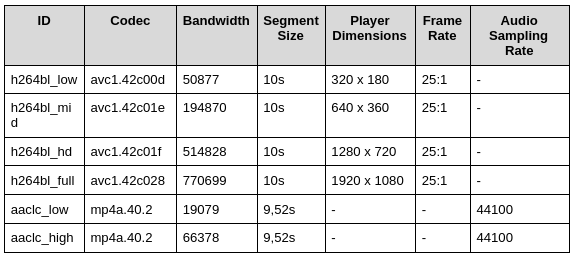
\includegraphics[width=0.9\linewidth,keepaspectratio]{MPDTable}
    \caption{mp4-main-multi-mpd-AV-NBS file analysis}
    \label{fig:MPD_Analysis}
\end{figure}
\FloatBarrier

The table above summarizes the information obtained from the 
"mp4-main-multi-mpd-AV-NBS.mpd" file and will serve as reference 
to answer the questions bellow.
\newline  

\Question{How many video and audio codecs are available?}

There are \underline{4 video codecs}: avc1.42c00d, avc1.42c01e, avc1.42c01f, avc1.42c028, and 

\underline{2 audio codecs}: mp4a.40.2 appearing in both aaclc\_low, aaclc\_high.

~\newline  

\Question{Which is the segment size?}

The duration of each segment is present on the \textit{SegmentList} tag of its 
\textit{Representation}: 
\begin{verbatim}
    <SegmentList timescale="1000" duration="10000">
\end{verbatim}

With \textit{"timescale"} being defined as a number of units per second.
As such, video segments are 10s long, while audio segments are 9.52s.

The \textit{"Period"} tag also indicates that it's total 
\textit{"duration="PT0H10M0.00S"}, (10 minutes), which adds up with the 
mentioned segment size given that each \textit{"SegmentList"} is made up of 60
\textit{"Segments"}.

~\newline  
\Question{Which audio and video data rates are available?}

In each \textit{Representation} tag, the \textit{"bandwidth"} field declares the
necessary data rate for continuous playout of its Segments.

That being said, the available data rates are:
\begin{itemize}
    \item Video:
        \begin{itemize}
            \item h264bl\_low: 50877 bps
            \item h264bl\_mid: 194870 bps
            \item h264bl\_hd: 514828 bps
            \item h264bl\_full: 770699 bps
        \end{itemize}
    \item Audio:
        \begin{itemize}
            \item aaclc\_low: 19079 bps
            \item aaclc\_high: 66378 bps
        \end{itemize}
\end{itemize}

~\newline  
\Question{Which options would you have for an available bandwidth of 500kbps, 1.5Mbps, 10Mbps?}

For convenience, we will refer to the segment ID's by 
video\_low/\_mid/\_hd/\_full and audio\_low/\_high.
~\newline

With an available bandwidth of 500kbps the best option would be:
\textbf{audio\_high + video\_mid} = 66kbps + 195kbps.


With a bandwidth of 1.5Mbps the best option possible would be the best one 
offered:
\textbf{audio\_high + video\_full} = 66kbps + 770kbps.

Likewise, with 10Mbps available the same thing happens.


~\newline
\Question{Play the video 
https://dash.akamaized.net/akamai/bbb\_30fps/bbb\_30fps.mpd, observe what happens for different controls (adaptation with different algorithms).
Use Wireshark to observe the playing of the video stream.
Describe the data transfer profile of the video stream, preferably 
with a plot.}

A similar analysis of the bbb\_30fps.mpd file was made, resulting in the table 
of figure \ref{fig:BBBMPD_Analysis}. 
For convenience sake, given that all codec's ID start with "bbb\_30fps\_", they 
will be reference only by the later part of their name.
\begin{figure}[h!]
    \centering
    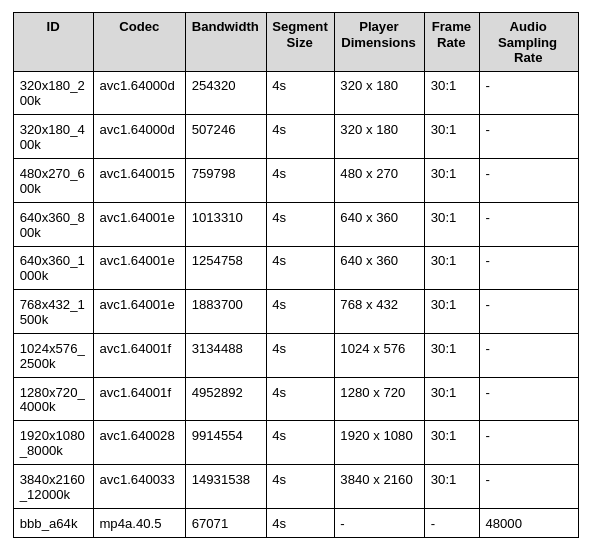
\includegraphics[width=0.9\linewidth,keepaspectratio]{BBBMPDTable}
    \caption{bbb\_30fps file analysis}
    \label{fig:BBBMPD_Analysis}
\end{figure}
\FloatBarrier

10 video codecs are available, with different bandwidths, all with segment 
sizes of 4s (duration: 120 on 
a timescale of 30):
\begin{verbatim}
   <SegmentTemplate duration="120" timescale="30" 
   media="$RepresentationID$/$RepresentationID$_$Number$.m4v" 
   startNumber="1" initialization="$RepresentationID$/$RepresentationID$_0.m4v"/>
\end{verbatim}
A single audio codec is available, also with segment size of 4s (duration: 
192512, on a timescale of 48000).
\begin{verbatim}
   <SegmentTemplate duration="192512" timescale="48000" 
   media="$RepresentationID$/$RepresentationID$_$Number$.m4a" 
   startNumber="1" initialization="$RepresentationID$/$RepresentationID$_0.m4a"/>
\end{verbatim}

Given that only 1 audio codec is available, only the image quality fluctuates 
in congestion scenarios. The maximum viewing experience,  
video codec 3840x2160 with bbb\_a64k audio, requires a bandwidth of 
14998609bps$\approx$\textbf{15Mbps} .


*TEMOS DE TENTAR PERCEBER, QUE FOI UMA COISA QUE A PROF FALOU, SE A CADA SEGMENTO O DASH SERVER RESPONDE COM DADOS, OU SE RECEBE VÁRIOS SEGMENTOS E SÓ DEPOIS RESPONDE COM DADOS, SE ESTES DADOS TÊM SEMPRE O MESMO TAMANHO*...

\newpage
\section*{Part 2: Bottleneck for quality degradation experiment} 

In order to force the DASH traffic to flow on a bottlenecked connection, an 
Iperf Server and Client were implemented within the following architecture:

\begin{figure}[h!]
    \centering
    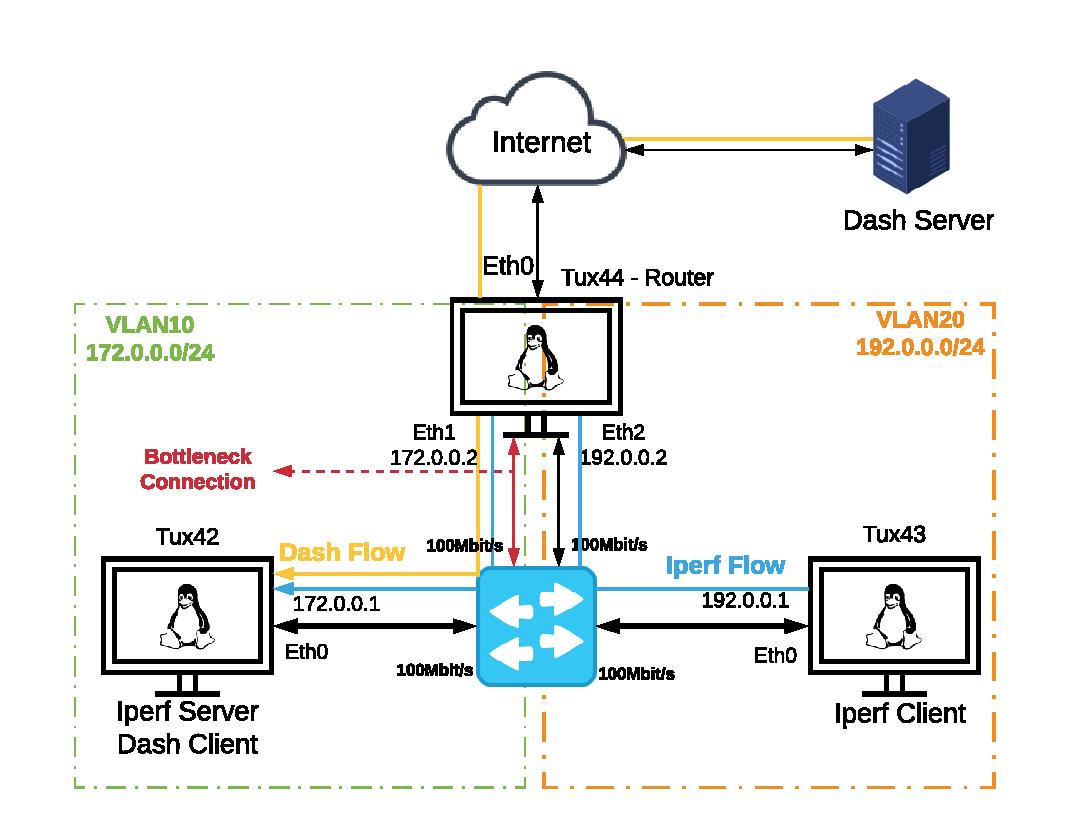
\includegraphics[width=0.9\linewidth,keepaspectratio]{NetworkArchi}
    \caption{Implemented Iperf and Dash architecture}
    \label{fig:Archi}
\end{figure}
\FloatBarrier

Iperf traffic flows from client to server, and since Tux43 and 42 are located in
different VLANs, this traffic needs to go through Tux44 (acting as a router).

Since Tux44 also functions as an outside router to the general Internet, Dash 
traffic (from Server to Client) is also forwarded through Tux44's Eth1, 
throttling the egress queue in Tux44's Eth1 connection.\\

Iperf traffic was generated on it's client side, \textbf{-c}, to the Iperf 
server (\textbf{172.0.0.1}) using the following command:
\begin{verbatim}
iperf3 -c 172.0.0.1 -t 0 -b 90M
\end{verbatim}
To note both the \textbf{-t 0} to ensure an infinite flow and \textbf{-b 90M} to
set a 90Mbit/s bandwidth.

~\newline
On the Iperf server side a simple command was used to specify it as a server:
\begin{verbatim}
iperf3 -s 
\end{verbatim}

~\newline
Is possible to observe the degradation of the DASH stream by simultaneously 
having a Iperf stream (from Tux43 to Tux42) and a DASH stream active:
\begin{figure}
    \centering
    \begin{minipage}{0.45\linewidth}
        \centering
        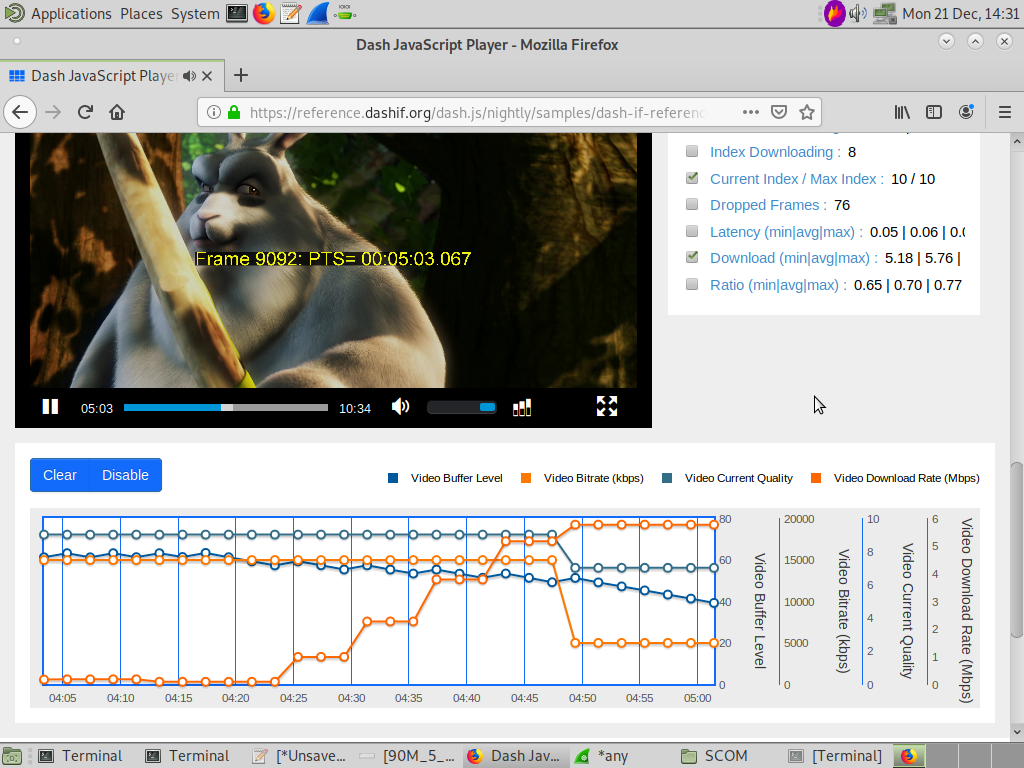
\includegraphics[width=0.9\linewidth]{GoodQuality} 
        \caption{Stream Quality: 10/10 - No Iperf}
    \end{minipage}\hfill
    \begin{minipage}{0.45\textwidth}
        \centering
        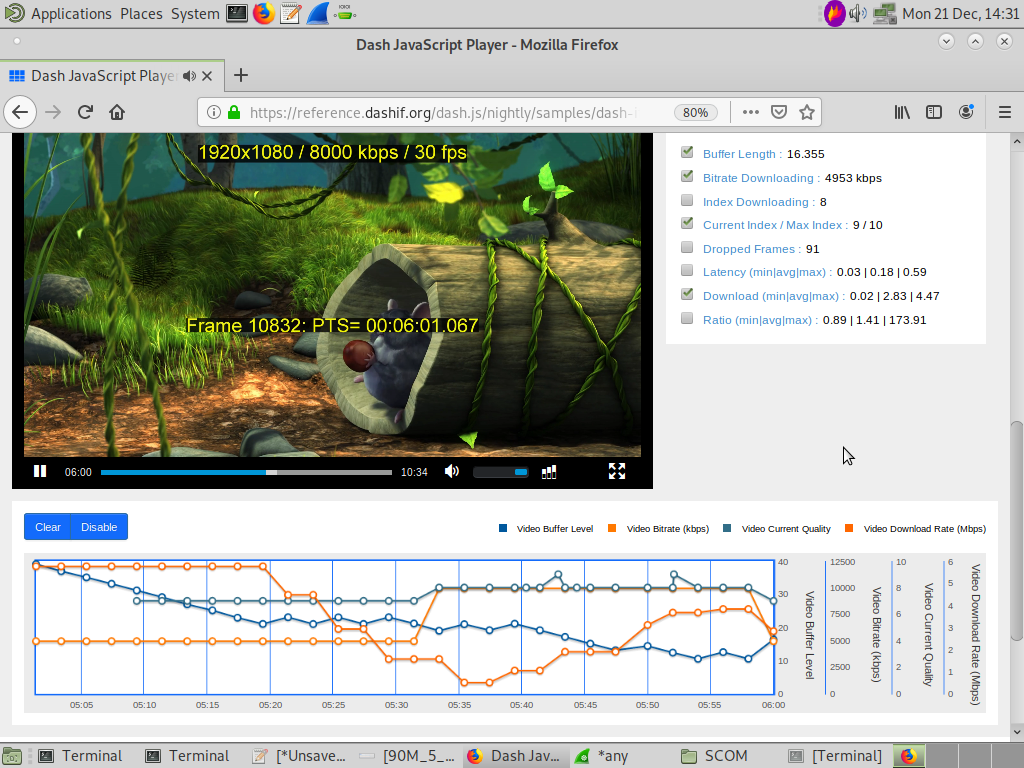
\includegraphics[width=0.9\linewidth]{PoorQuality}
        \caption{Stream Quality: 8/10 - 90M Iperf}
    \end{minipage}
\end{figure}
\FloatBarrier	
~\newline

With an active \textbf{UDP} Iperf stream, the DASH player behaved as follows:


"Finish the iperf UDP traffic before the end of the stream, and observe what happens." 

"Show your observations using the wireshark trace analysis tool, mark the 
timestamps at which you added and changed cross traffic. 
Justify what you are seeing."

\Question{Observe the behaviour of the video player:}
\begin{itemize}

    \item \Question{Which data rates is the player choosing?}
        
        Without a UDP Iperf stream the player chooses the maximum quality 
        available: \textbf{10/10 - 3840x2160 - 14931kbps}. 
        
        With UDP cross traffic, these data rates decrease, as does the video 
        quality, to a resolution of \textbf{9/10 - 1920x1080 - 9914kbps}, 
        and sometimes even \textbf{8/10 - 1280x720 - 4952kbps}. 

        Note that, as showed in figure \ref{fig:UDPDASH_8to9}, even with 
        Iperf cross traffic, the DASH client still adapts when possible 
        (increasing it's quality from 8 to 9).
    \begin{figure}[h!]
        \centering
        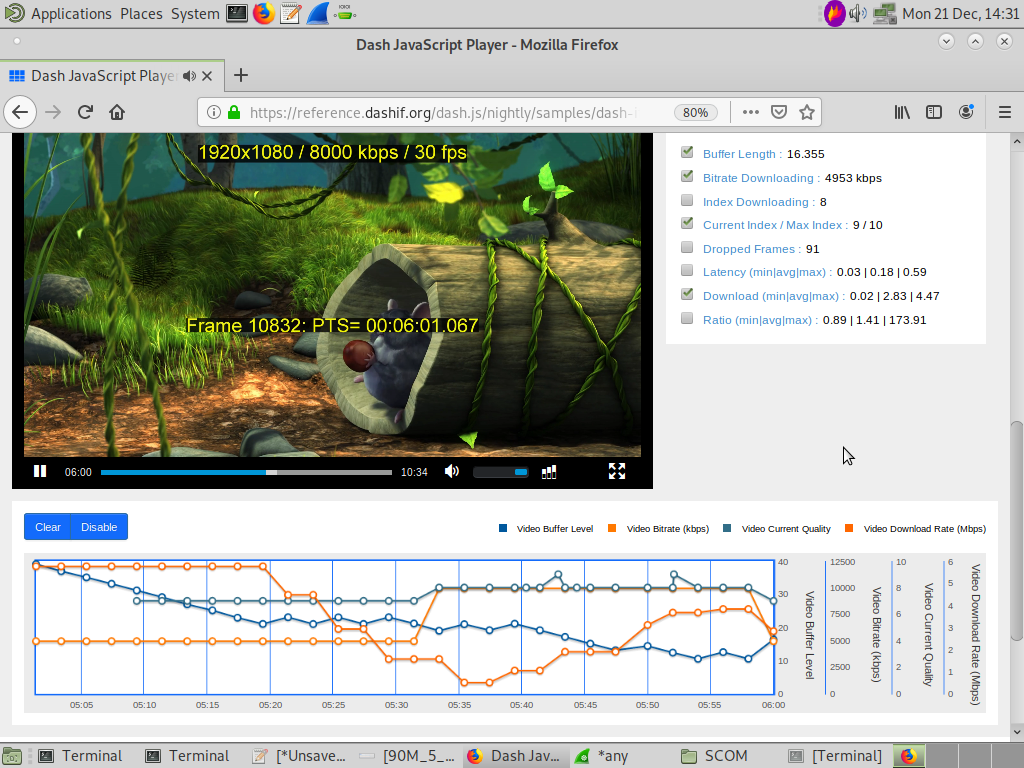
\includegraphics[width=0.8\linewidth,keepaspectratio]{PoorQuality}
        \caption{DASH client quality increasing from 8 back to a 9}
        \label{fig:UDPDASH_8to9}
    \end{figure}
    \FloatBarrier
        
    \item \Question{How often are segments requested?}
        <++>
    \item \Question{How does the player tell the server which rate to use?}
        <++>

\end{itemize}

With an active \textbf{TCP} Iperf stream, the DASH player behaved as follows:

"Show your observations using the wireshark trace analysis tool, mark the 
timestamps at which you added and changed cross traffic. 
Justify what you are seeing."

"Observe the behaviour of the video player."
\begin{itemize}

    \item Which data rates is the player choosing?"

    \item "How often are segments requested?":

    \item "How does the player tell the server which rate to use?"

\end{itemize}

\Question{Were does the behaviour differer for TCP and UDP cross traffic? How? 
Why? Did you expect this behaviour?} 

Given TCP's congestion avoidance and it's congestion window scheme, a different 
behaviour for it's cross traffic was expected.
Whilst UDP's cross traffic simply tries to occupy the entire available 
bandwidth, with no regard to traffic congestion, TCP's cross traffic "backs-off"
once it reaches a timeout packet and enters \textit{slow-start}.

~\newline
The impact of this in the DASH stream is minimal, even though the DASH client 
is aware of the TCP cross traffic (rise of the video download rate), no actual
codec change is registered. 
Hence, the DASH client quality is not affected by Iperf's TCP cross traffic.

Such can be confirmed by the figure \ref{fig:TCPDASH_Drop}, where incoming 
Iperf traffic throughput oscillates, due to TCP's "back-off" between 
45-90Mbit/s, not being consistently high enough to compromise DASH's quality.
\begin{figure}[h!]
    \centering
    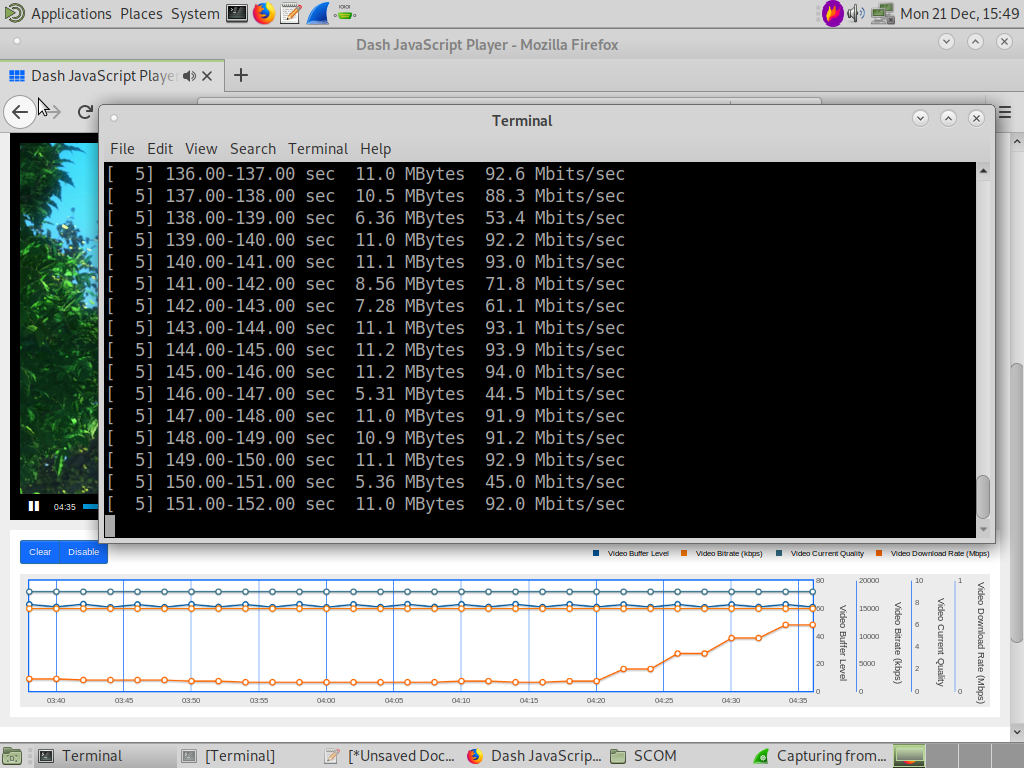
\includegraphics[width=0.9\linewidth,keepaspectratio]{TCPDASH_Drop}
    \caption{Iperf Incoming Traffic and DASH Client impact during both flows}
    \label{fig:TCPDASH_Drop}
\end{figure}
\FloatBarrier

\section*{Part 3: Bandwidth reservation for video flow} 

In order to safeguard the DASH flow from degradation due to bandwidth sharing,
a HTB (Hierarchy Token Bucket) queueing policy was implemented on Tux44, 
reserving a minimum guaranteed bandwidth for DASH traffic.

Using the Linux traffic control tool (\textbf{tc}) a HTB queueing discipline 
with the handle 1: was attached to Tux44's Eth1:
\begin{verbatim}
tc qdisc add dev eth1 root handle 1: htb default 12
\end{verbatim}

A general overview of this hierarchy queueing discipline can be seen on figure 
\ref{fig:HTBHierarchy}.

\begin{figure}[h]
    \centering
    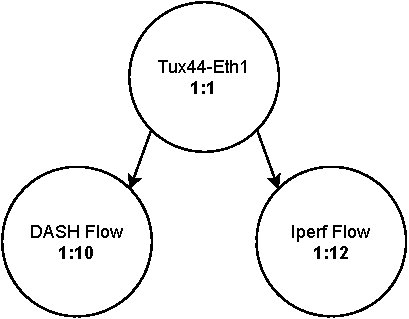
\includegraphics[width=0.3\linewidth,keepaspectratio]{HTBHierarchy}
    \caption{Implemented HTB Hierarchy on TUX44's Eth1}
    \label{fig:HTBHierarchy}
\end{figure}
\FloatBarrier

3 TC classes were created for the different types of traffic and their 
requirements:
\begin{verbatim}
tc class add dev eth1 parent 1: classid 1:1 htb rate 100mbit ceil 100mbit 
tc class add dev eth1 parent 1:1 classid 1:10 htb rate 20mbit ceil 100mbit
tc class add dev eth1 parent 1:1 classid 1:12 htb rate 80mbit ceil 80mbit
\end{verbatim}
(rate: guaranteed available bandwidth for that class; 
~\\
ceil: highest rate a class can reach, if it's parent has bandwidth to 
spare).

~\\
The 1st class is considered a root class, with the following ones being it's 
leafs.
Class 1:10 (DASH flow) has a guaranteed bandwidth of 20mbit but can reach
100mbit if the root class has bandwidth to spare while 
Class 1:12 (default and Iperf) has a guaranteed and maximum bandwidth of 80mbit.

A value of 20mbit was chosen for the DASH traffic, since it's maximum codec only
requires 15mbit.


~\\
To associate the correct packets to their traffic classes, the following 
filter was applied: 
\begin{verbatim}
tc filter add dev eth1 protocol ip parent 1:0 prio 1 u32 match ip src 194.210.238.81 flowid 1:10
\end{verbatim}
Associating the packets on Tux44's Eth1, with a source IP of 194.210.238.81 
(DASH Server's IP) to the class 1:10 and it's requirements.

~\\
\Question{Re-run the experiments with cross traffic that you performed before, 
document them using the TCP throughput plots, and explain the observations.} 

~\\
With this HTB queueing policy in place the DASH flow is never compromised, 
as depicted in figure \ref{fig:UDPTCDASH} regardless of the protocol of the 
Iperf generated traffic (TCP or UDP).

\begin{figure}[h!]
    \centering
    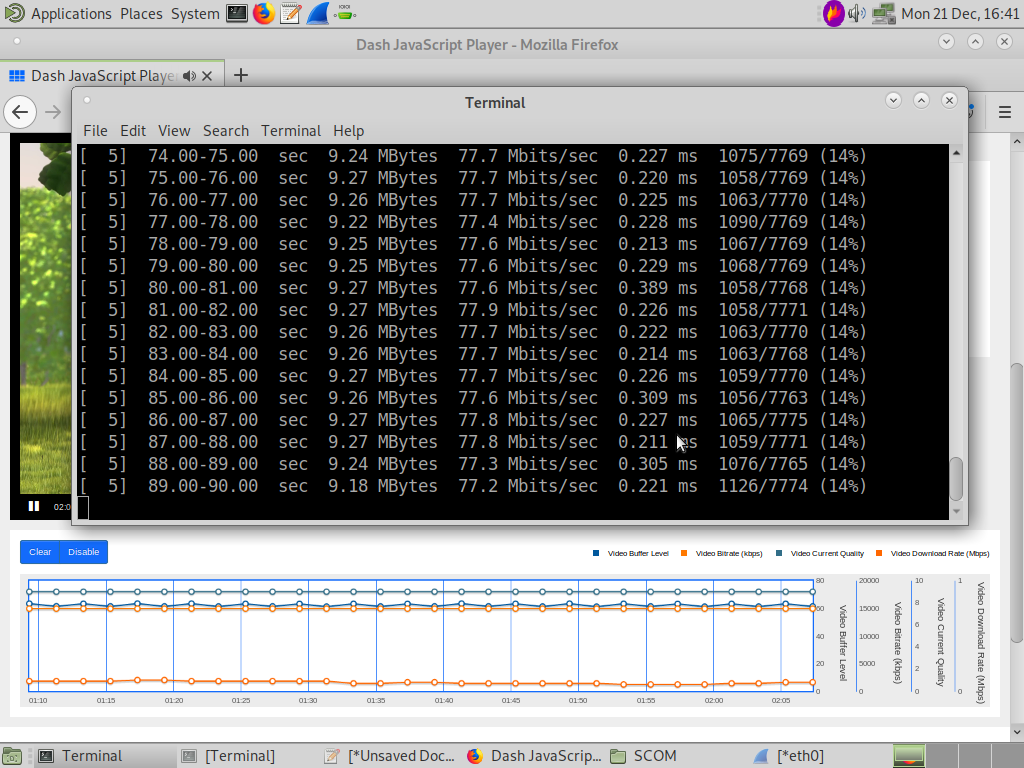
\includegraphics[width=0.9\linewidth,keepaspectratio]{UDPTCDASH}
    \caption{DASH client constant quality with UDP Iperf traffic active, thanks 
             to HTB policy} 
    \label{fig:UDPTCDASH}
\end{figure}
\FloatBarrier

The differences between both protocols, on the Iperf client side, still 
remained, with the aforementioned TCP congestion control mechanisms still 
present, as depicted on figure 
\ref{fig:TCPIperf_TC}, and the immediate and persistent total bandwidth usage of
UDP, as seen on figure \ref{fig:UDPIperf_TC}.

Note that Iperf's client sends 90Mbit, and not the imposed limit of 80M since 
the this limitation is only present on the egress Tux44's Eth1 connection, and 
not on the Iperf client itself.
Again, that limitation can be seen on the server's side on figure 
\ref{fig:UDPTCDASH}.

\begin{figure}[h!]
    \centering
    \begin{minipage}{0.45\linewidth}
        \centering
        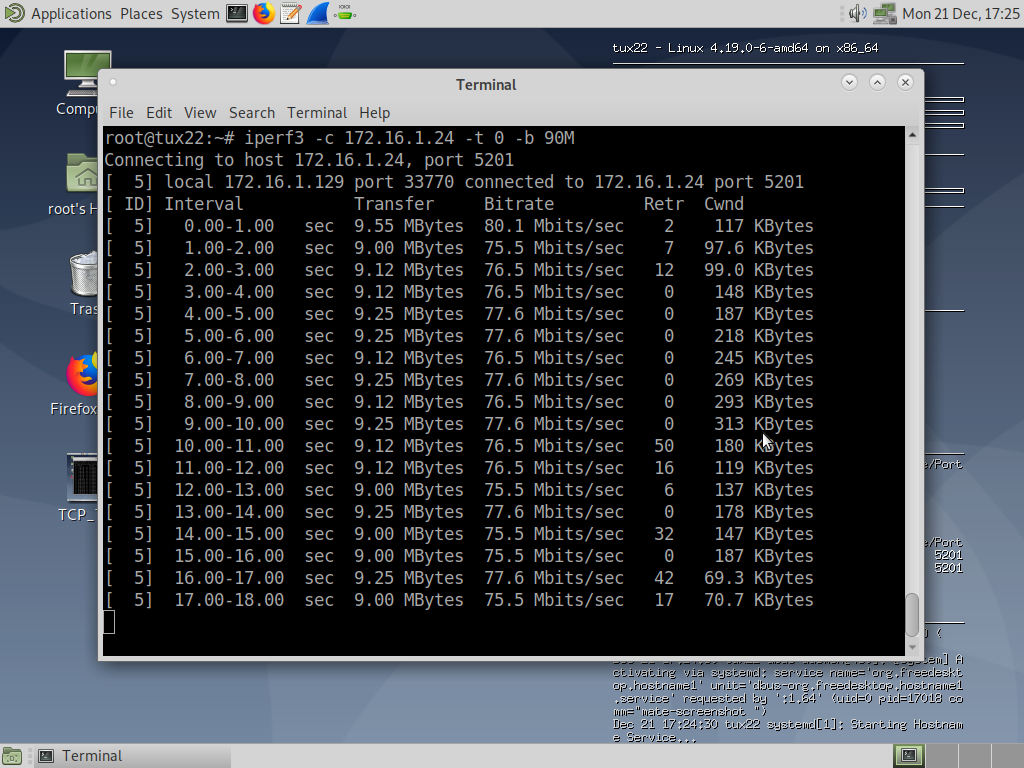
\includegraphics[width=1.2\textwidth]{TCPIperf_TC} 
        \caption{TCP Iperf traffic with HTB policy}
        \label{fig:TCPIperf_TC}
    \end{minipage}\hfill
    \begin{minipage}{0.45\textwidth}
        \centering
        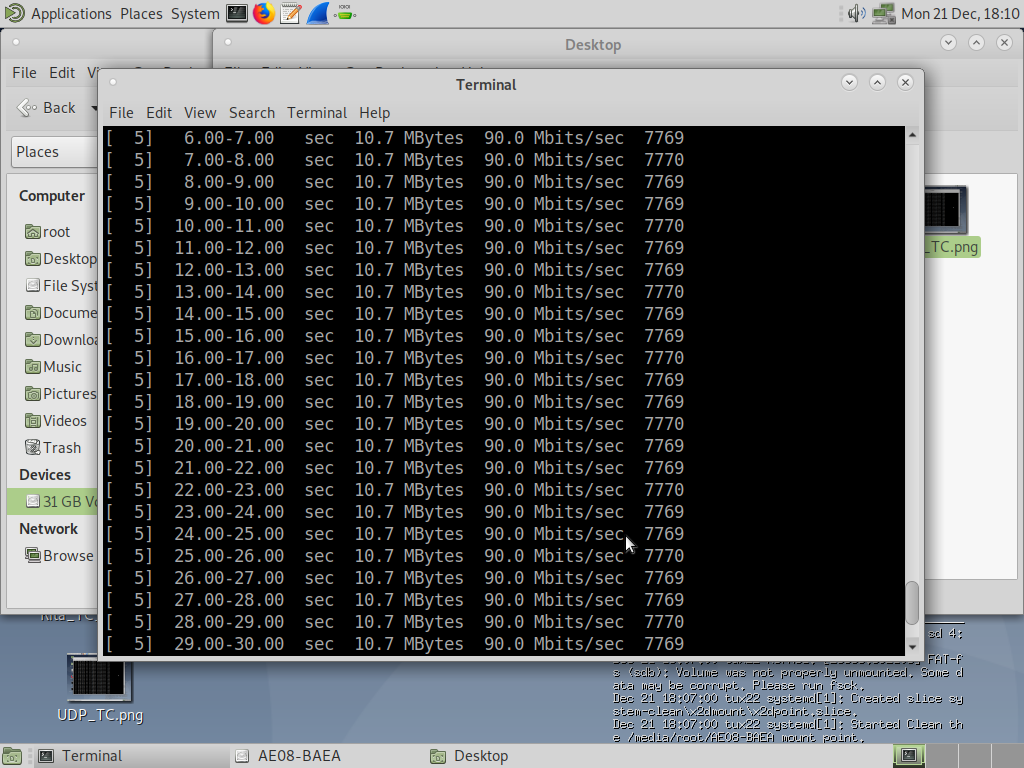
\includegraphics[width=1.2\linewidth]{UDPIperf_TC}
        \caption{UDP Iperf traffic with HTB policy}
        \label{fig:UDPIperf_TC}
    \end{minipage}
\end{figure}
\FloatBarrier	

*FOTO DAS ESTATISTICAS, A REFERIR AS CENAS MAIS EVIDENTES*
\begin{figure}[h!]
    \centering
    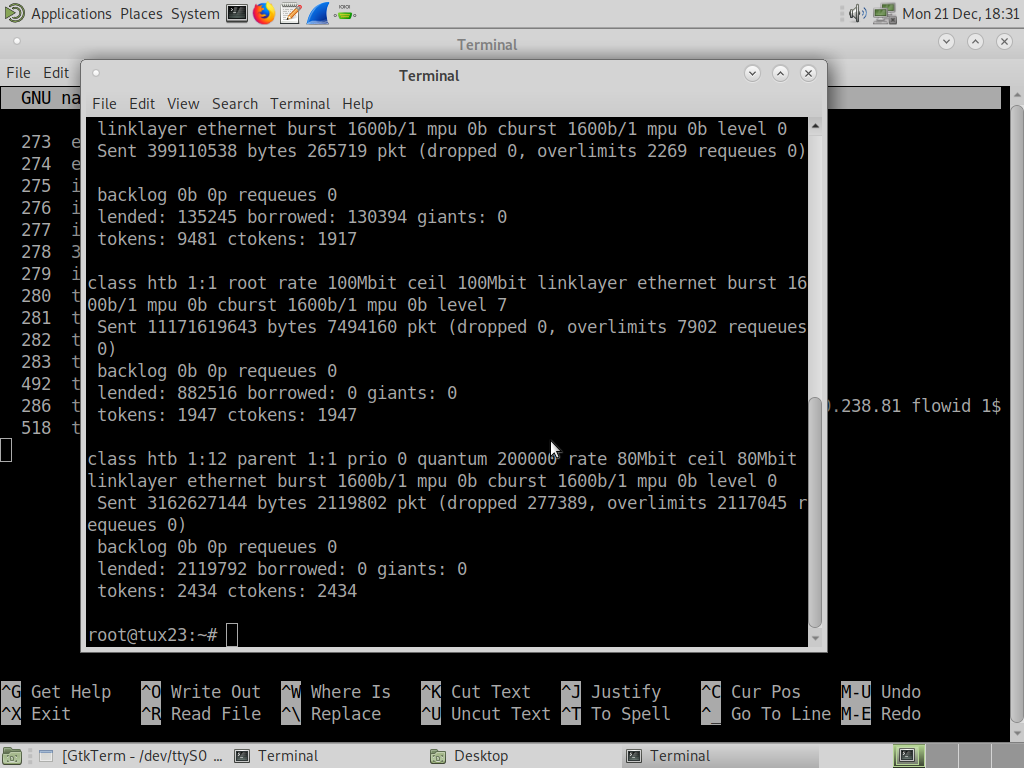
\includegraphics[width=0.9\linewidth,keepaspectratio]{TCStats}
    \caption{TC stats - output of: tc -s -d class show dev eth1}
    \label{fig:TCStats}
\end{figure}
\FloatBarrier

\end{document}

